
\documentclass[withoutpreface,bwprint]{cumcmthesis} %去掉封面与编号页
\usepackage{url}%引用网站
\usepackage{cite}%引用参考文献
\usepackage{graphicx}
\title{基于主要模型对关键词的研究}
%\tihao{A}
%\baominghao{4321}
%\schoolname{北京理工大学珠海学院}
%\yearinput{2021}
%\monthinput{08}
%\dayinput{10}

\begin{document}

\maketitle%与上面的\title对应
\begin{abstract}


TOPS:小背景

%\textbf{}:加粗	
\textbf{针对问题一},
			
\textbf{针对问题二},

\textbf{针对问题三},

\keywords{关键词1\quad  关键词2\quad   关键词3\quad   关键词4\quad 关键词5}
%\keywords:关键词;\quad:空格
\end{abstract}

%\section{}-subsection{}-subsubsection{}:标题1-3级
\section{问题重述}
\subsection{背景}

TOPS:大背景:写够半页(让问题重述部分差不多一页)(删掉此句话)

\subsection{重述}
结合以上情况,建立数学模型解决以下问题:

\begin{enumerate}
\item 	
	
\item 
	
\item 
\end{enumerate}

\newpage%\新一页
\section{模型的假设}
TOPS:这部分写4-6个(删掉此句话)

针对本文题目,提出以下假设建模思路:
	
\begin{itemize}
	\item 
	\item 
	\item 
	\item 
	\item
\end{itemize}
	
\section{符号说明}
这部分不要过页(删掉此句话)
\begin{center}%置中
\begin{tabular}{cc}
\toprule[1pt] 
\makebox[0.15\textwidth][c]{符号} & \makebox[0.4\textwidth][c]{说明} \\  
\hline
            $T_i$&小温区温度\\
            $T_i$&小温区温度\\    
\bottomrule[1pt]
\end{tabular}
\end{center}

\newpage
\section{问题分析}
TOPS:这部分写差不多一页(删掉此句话)
\subsection{问题一分析}
对于问题一,

\subsection{问题二分析} 
对于问题二,

\subsection{问题三分析}
对于问题三,

\subsection{问题四分析}
对于问题四,

\newpage
	
\section{模型的建立与求解}

\subsection{二级标题}

\subsubsection{三级标题}


\subsubsection{列表环境}
\begin{enumerate}
	\item 
	
	\item 	
\end{enumerate}


\begin{itemize}
	\item[(a)] 
	
	
	\item[(b)] 	
\end{itemize}


\begin{itemize}
	\item 
	\item 
\end{itemize}
	
\subsubsection{图}	
\begin{figure}[h]%[h]:固定作用
	\centering%置中
	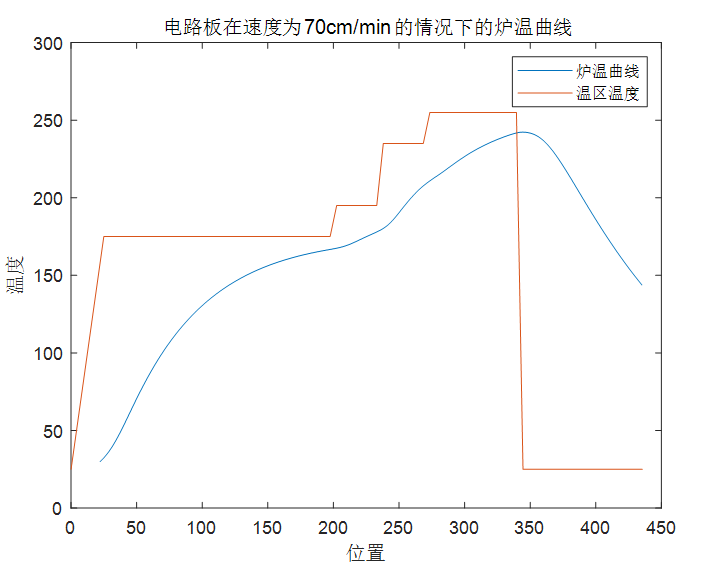
\includegraphics [scale=0.5]{figures/1.png}
	\caption{图名} 
	\label{fig:1}
\end{figure}

TOPS:如何引用看这里:图\ref{fig:1}

\newpage

\subsubsection{表}

\begin{table}[!htbp]
	\caption{表名}	\centering
	\begin{tabular}{c c}
		\hline \multicolumn{1}{c} { 焊接区域中心温度} & 时间 $(\mathrm{s})$ \\
		\hline $30^{\circ} \mathrm{C}$ & 0 \\
		$150^{\circ} \mathrm{C}$ & $t_{1}$ \\
		$190^{\circ} \mathrm{C}$ & $t_{2}$ \\
		\hline
		\label{tab:1}
	\end{tabular}
\end{table}

TOPS:如何引用看这里:表\ref{tab:1}

\subsubsection{公式}

$\alpha^2+\beta^2=\gamma^2$

$$ \alpha^2+\beta^2=\gamma^2$$

\begin{equation}\nonumber
	\alpha^2+\beta^2=\gamma^2
\end{equation}

\begin{equation}
	\alpha^2+\beta^2=\gamma^2 \label{1}
\end{equation}

\begin{equation}
	a+b=c \label{2}
\end{equation}

TOPS:如何引用看这里:公式\eqref{1}和公式\eqref{2}
\newpage

\section{误差分析}

有时间再做(没时间删去,影响不大)

\section{模型的评价}
	
\subsection{模型的优点}

\begin{itemize}
	
\item[(1)] 

\item[(2)] 

\item[(3)] 

\end{itemize}	
	
\subsection{模型的缺点}
	
\begin{itemize}
	
	\item[(1)] 
	
	\item[(2)] 
	
	\item[(3)] 
	
\end{itemize}	

\newpage
    %参考文献
\begin{thebibliography}{9}%宽度9
	
	\setlength{\itemsep}{-1mm}
	\bibitem{bib:one} 	
	\bibitem{bib:two} 
	\bibitem{bib:three} 
    \bibitem{bib:four} 
    \bibitem{bib:five} 
    \bibitem{bib:six} 
    \bibitem{bib:seven} 	
    \bibitem{bib:eight} 
    \bibitem{bib:nine} 刘润幸. 使用SPSS作多变量观察值的ROC曲线分析[J]. 中国公共卫生, 2003, 19(9): 1151-1152.
    

TOPS:如何引用——看这\textsuperscript{\cite{bib:one}}

\end{thebibliography}	
\newpage
%附录
\appendix
	
\section{程序代码}
\begin{lstlisting}[language=matlab]
	kk=2;[mdd,ndd]=size(dd);
	while ~isempty(V)
	[tmpd,j]=min(W(i,V));tmpj=V(j);
	for k=2:ndd
	[tmp1,jj]=min(dd(1,k)+W(dd(2,k),V));
	tmp2=V(jj);tt(k-1,:)=[tmp1,tmp2,jj];
	end
	tmp=[tmpd,tmpj,j;tt];[tmp3,tmp4]=min(tmp(:,1));
	if tmp3==tmpd, ss(1:2,kk)=[i;tmp(tmp4,2)];
	else,tmp5=find(ss(:,tmp4)~=0);tmp6=length(tmp5);
	if dd(2,tmp4)==ss(tmp6,tmp4)
	ss(1:tmp6+1,kk)=[ss(tmp5,tmp4);tmp(tmp4,2)];
	else, ss(1:3,kk)=[i;dd(2,tmp4);tmp(tmp4,2)];
	end;end
	dd=[dd,[tmp3;tmp(tmp4,2)]];V(tmp(tmp4,3))=[];
	[mdd,ndd]=size(dd);kk=kk+1;
	end; S=ss; D=dd(1,:);
\end{lstlisting}

\section{支撑材料}

TOPS:有支撑材料就写(要和文件名一致),没有就删去这部分

\begin{enumerate}
	\item 	
	
	\item 
	
	\item 
\end{enumerate}

\end{document}

